
\documentclass[11pt]{article}

\usepackage[margin=1.05in]{geometry}
\usepackage[T1]{fontenc}
\usepackage[utf8]{inputenc}
\usepackage{lmodern}
\usepackage{amsmath,amssymb,amsfonts,amsthm,mathtools}
\usepackage{bm}
\usepackage{enumitem}
\usepackage{hyperref}
\usepackage[nameinlink,capitalise]{cleveref}
\usepackage{tikz}
\usetikzlibrary{decorations.pathmorphing,arrows.meta,calc,positioning}

\hypersetup{
  colorlinks=true,
  linkcolor=blue!60!black,
  citecolor=blue!60!black,
  urlcolor=blue!60!black,
  pdftitle={2026 Cargese Lectures: Defects in Quantum Field Theory},
  pdfauthor={Zohar Komargodski}
}

\setlist[itemize]{topsep=2pt,itemsep=2pt,parsep=2pt}
\setlist[enumerate]{topsep=2pt,itemsep=2pt,parsep=2pt}

\newtheorem{theorem}{Theorem}[section]
\newtheorem{proposition}[theorem]{Proposition}
\newtheorem{lemma}[theorem]{Lemma}
\newtheorem{definition}[theorem]{Definition}
\newtheorem{exercise}[theorem]{Exercise}
\newtheorem{remark}[theorem]{Remark}
\newtheorem{example}[theorem]{Example}

\newcommand{\R}{\mathbb{R}}
\newcommand{\Z}{\mathbb{Z}}
\newcommand{\C}{\mathbb{C}}
\newcommand{\dd}{\mathrm{d}}
\newcommand{\cD}{\mathcal{D}}
\newcommand{\cO}{\mathcal{O}}
\newcommand{\cA}{\mathcal{A}}
\newcommand{\cC}{\mathcal{C}}
\newcommand{\cH}{\mathcal{H}}
\newcommand{\cL}{\mathcal{L}}
\newcommand{\cM}{\mathcal{M}}
\newcommand{\cN}{\mathcal{N}}
\newcommand{\what}{\widehat}
\newcommand{\vev}[1]{\left\langle #1\right\rangle}
\newcommand{\defeq}{\equiv}
\newcommand{\vol}{\operatorname{vol}}
\newcommand{\sgn}{\operatorname{sgn}}
\newcommand{\id}{\mathbf{1}}

\title{2026 Cargese Lectures:\\ Defects in Quantum Field Theory}
\author{Zohar Komargodski\\
\small Simons Center for Geometry and Physics, Stony Brook University}
\date{Cargese 2026}

\begin{document}
\maketitle

\begin{center}
\begin{minipage}{0.82\textwidth}
\small\itshape
These preliminary notes accompany the 2026 Cargese lectures and have not yet
undergone a complete editorial and bibliographic review.
\end{minipage}
\end{center}

\medskip

\tableofcontents
\newpage


\section{Defects as extended operators}

\subsection{What is a defect?}

Let $X$ be a $d$-dimensional Euclidean spacetime.  A $p$-dimensional defect is an extended operator supported on an embedded submanifold
\begin{equation}
  \Sigma_p \hookrightarrow X_d .
\end{equation}
Its codimension is
\begin{equation}
  q=d-p .
\end{equation}
The defect may be defined by modifying the path integral near $\Sigma_p$, by imposing singular boundary conditions around $\Sigma_p$, by adding degrees of freedom living on $\Sigma_p$, or by inserting a topological operator.  The most common examples are:
\begin{itemize}
  \item local operators: $p=0$;
  \item line defects: $p=1$, such as Wilson lines, impurities, worldlines of external charged particles;
  \item surface defects: $p=2$;
  \item boundaries or interfaces: $p=d-1$;
  \item domain walls, including topological symmetry defects.
\end{itemize}

A useful definition is operational.  A defect $\cD(\Sigma)$ is something that can be inserted into correlation functions:
\begin{equation}
  \vev{\cD(\Sigma)\, \cO_1(x_1)\cdots \cO_n(x_n)} .
\end{equation}
If the insertion changes the theory only in a small tubular neighborhood of $\Sigma$, it is local as an extended operator.  The tubular neighborhood is useful because it lets us replace a defect by boundary conditions on the boundary of the tube.  For a line defect in $d=3$, the boundary of a small tube is $S^1\times \R$.

\begin{figure}[htbp]
\centering
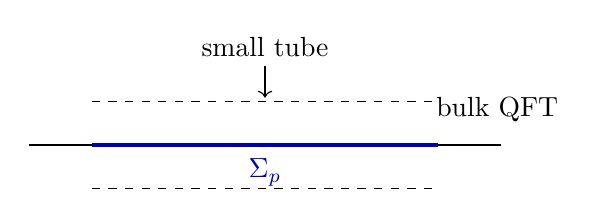
\begin{tikzpicture}[scale=1.0]
  \draw[thick] (-3,0) -- (3,0);
  \draw[ultra thick,blue!70!black] (-2.2,0) -- (2.2,0);
  \draw[dashed] (-2.2,0.55) -- (2.2,0.55);
  \draw[dashed] (-2.2,-0.55) -- (2.2,-0.55);
  \node[blue!70!black] at (0,-0.35) {$\Sigma_p$};
  \node at (2.95,0.45) {bulk QFT};
  \draw[->] (0,1.0) -- (0,0.6);
  \node at (0,1.25) {small tube};
\end{tikzpicture}
\caption{A defect can be defined by excising a tubular neighborhood and imposing boundary conditions on the tube.}
\end{figure}

\subsection{Defect actions and defect Hilbert spaces}

A defect may have intrinsic degrees of freedom.  In that case the microscopic description often takes the form
\begin{equation}
  S_{\rm tot}=S_{\rm bulk}+S_{\rm def}[\chi;X^*\Phi]+\int_{\Sigma_p}\sum_I \lambda^I \widehat{\mathcal O}_I .
\end{equation}
Here $\Phi$ denotes bulk fields, $X^*\Phi$ their pullback to $\Sigma_p$, and $\chi$ possible defect-local fields.  The hatted operators are defect operators.

For a line defect, quantization along the line produces a one-dimensional defect Hilbert space, but it is usually not an autonomous Hilbert space: it is coupled to the bulk.  The line supports a one-dimensional operator algebra consisting of operators inserted on the line.  At a defect conformal fixed point this becomes a one-dimensional conformal quantum mechanics.

\subsection{Topological versus conformal versus generic defects}

There are three logically distinct notions.
\begin{enumerate}
  \item A \emph{topological defect} can be deformed continuously without changing correlation functions, as long as it does not cross other operator insertions.  It has no local stress response to shape deformations.
  \item A \emph{conformal defect} is not topological, but preserves the conformal transformations that leave its shape invariant.  A flat $p$-plane in a $d$-dimensional CFT preserves $SO(p+1,1)\times SO(q)$.
  \item A \emph{generic defect} preserves only translations/rotations along the defect, or even less.  Under defect RG flow it may approach a conformal defect in the infrared.
\end{enumerate}

These are not mutually exclusive.  A topological defect in a CFT is automatically conformal, but it is much more constrained than a generic conformal defect.  The key diagnostic is the displacement operator, introduced below.

\section{Topological defects and generalized symmetry}

This section follows the point of view of generalized global symmetry and non-invertible symmetry.  A particularly pedagogical reference is Shao's TASI lectures on non-invertible symmetries, which emphasize that topological defects are often the right language for symmetry.

\subsection{Topological invariance and the displacement operator}

Consider an infinitesimal deformation of the embedding $X^\mu(\sigma)$ of a defect:
\begin{equation}
  X^\mu(\sigma)\longrightarrow X^\mu(\sigma)+\delta X^\mu(\sigma) .
\end{equation}
Tangential deformations are reparametrizations.  The physical deformations are normal to $\Sigma$.  Let $n_i^\mu$, $i=1,\dots,q$, be an orthonormal frame of the normal bundle, and write
\begin{equation}
  \delta X^\mu=\delta X^i n_i^\mu+\text{tangential} .
\end{equation}
The response to a shape deformation defines the displacement operator $D_i$:
\begin{equation}
  \delta \log \vev{\cD(\Sigma)\cdots}
  =-\int_\Sigma \dd^p\sigma\,\sqrt{\gamma}\,\delta X^i(\sigma)
  \frac{\vev{D_i(\sigma)\cD(\Sigma)\cdots}}{\vev{\cD(\Sigma)\cdots}}+\text{contact terms} .
  \label{eq:shapevariation}
\end{equation}

\begin{definition}
A defect is topological if all correlation functions are invariant under smooth deformations of $\Sigma$ that do not cross insertions.  Equivalently, the displacement operator vanishes in correlation functions up to contact terms with crossed operators.  In cohomological/topological theories one often weakens this to $D_i=\{Q,\Lambda_i\}$.
\end{definition}

For symmetry defects in ordinary QFT, the displacement operator vanishes because the defect is built from a conserved current.  For non-topological conformal defects $D_i$ is a genuine protected operator.

\subsection{Ordinary symmetry defects}

Let a QFT have a global symmetry group $G$.  For a connected ordinary symmetry with conserved current $J^\mu_a$, the conserved charge on a Cauchy surface $M^{d-1}$ is
\begin{equation}
  Q_a(M)=\int_{M^{d-1}} \star J_a .
\end{equation}
For $g=\exp(i\alpha^a T_a)$ one writes formally
\begin{equation}
  U_g(M)=\exp\left(i\alpha^a Q_a(M)\right) .
\end{equation}
The conservation equation $\dd \star J_a=0$ implies that $U_g(M)$ is invariant under deformations of $M$ that do not cross charged insertions.  Thus $U_g(M)$ is a codimension-one topological defect.

If $M$ is deformed across a local operator $\cO(x)$ transforming in representation $R$, then
\begin{equation}
  U_g(M)\,\cO(x)=R(g)\cO(x)\,U_g(M)
\end{equation}
where the equation is understood inside correlation functions and the ordering records on which side of $M$ the operator lies.

\begin{figure}[htbp]
\centering
\begin{tikzpicture}[scale=1.0]
  \draw[->,thick] (-3,0) -- (3,0) node[right] {$x$};
  \draw[thick,red!70!black] (-1.1,-1.2) -- (-1.1,1.2);
  \draw[thick,red!70!black,dashed] (1.1,-1.2) -- (1.1,1.2);
  \filldraw[black] (0,0) circle (2pt) node[below right] {$\cO$};
  \draw[->,red!70!black] (-0.7,1.0) -- (0.7,1.0);
  \node[red!70!black] at (-1.55,1.35) {$U_g$};
  \node[red!70!black] at (1.55,1.35) {$U_g$};
\end{tikzpicture}
\caption{Dragging a symmetry defect through a charged operator implements the symmetry action.}
\end{figure}

The fusion law is the group law:
\begin{equation}
  U_g\times U_h=U_{gh},\qquad U_g^{-1}=U_{g^{-1}} .
\end{equation}
This invertibility is the defining feature of ordinary group-like symmetries.

\subsection{Higher-form symmetry defects}

A $q$-form global symmetry in $d$ dimensions acts on $q$-dimensional charged operators.  It has a conserved $(q+1)$-form current $J_{q+1}$ satisfying
\begin{equation}
  \dd \star J_{q+1}=0 .
\end{equation}
For an Abelian group, the symmetry defect is supported on a closed codimension-$(q+1)$ manifold $M^{d-q-1}$:
\begin{equation}
  U_\alpha(M^{d-q-1})=\exp\left(i\alpha\int_{M^{d-q-1}}\star J_{q+1}\right) .
\end{equation}
A charged $q$-dimensional operator $W(C^q)$ is detected by linking:
\begin{equation}
  U_\alpha(M) W(C)=e^{i\alpha Q\,\operatorname{Link}(M,C)} W(C) .
\end{equation}

\begin{example}[Maxwell theory in four dimensions]
Free Maxwell theory has electric and magnetic one-form symmetries with currents
\begin{equation}
  J_e=\frac{1}{e^2}F,\qquad J_m=\frac{1}{2\pi}\star F .
\end{equation}
The charged operators are Wilson and 't Hooft lines.  The symmetry defects are codimension-two surfaces linking these lines.
\end{example}



\subsection{Topological operators as algebraic data}

Once defects are topological, their correlation functions depend only on topology.  Bringing two parallel topological defects close together defines a fusion product.  For invertible symmetry defects fusion gives a group.  More generally,
\begin{equation}
  \cN_a\times \cN_b=\sum_c N_{ab}^{\phantom{ab}c}\,\cN_c,
  \qquad N_{ab}^{\phantom{ab}c}\in\Z_{\ge 0} .
  \label{eq:fusionring}
\end{equation}
Associativity implies
\begin{equation}
  \sum_e N_{ab}^{\phantom{ab}e}N_{ec}^{\phantom{ec}f}
  =\sum_e N_{ae}^{\phantom{ae}f}N_{bc}^{\phantom{bc}e} .
  \label{eq:fusionassocnumbers}
\end{equation}
However, \eqref{eq:fusionassocnumbers} is only the decategorified shadow of the real structure.  The full data of topological lines in a two-dimensional QFT are categorical.  Under the usual finiteness and semisimplicity assumptions, topological line defects form a fusion category.  The simple objects are the simple topological lines, the tensor product is fusion of parallel lines, and the unit object is the invisible line $\id$.

The slogan for the blackboard is:
\begin{equation}
  \text{fusion rules are not enough; one also needs junction spaces and associators.}
\end{equation}
This is the same distinction as between knowing which intermediate channels appear in an OPE and knowing the crossing matrices that relate different OPE channels.

\paragraph{Junction vector spaces.}
For simple topological lines $a,b,c$, the basic local operators are trivalent junctions.  They form finite-dimensional vector spaces
\begin{equation}
  V_{ab}^{\phantom{ab}c}\defeq \operatorname{Hom}(a\otimes b,c),
  \qquad
  V_{c}^{\phantom{c}ab}\defeq \operatorname{Hom}(c,a\otimes b) .
  \label{eq:junctionspaces}
\end{equation}
The integer appearing in the fusion rule is
\begin{equation}
  N_{ab}^{\phantom{ab}c}=\dim V_{ab}^{\phantom{ab}c} .
\end{equation}
A basis vector in $V_{ab}^{\phantom{ab}c}$ is drawn as a trivalent topological junction:
\begin{center}
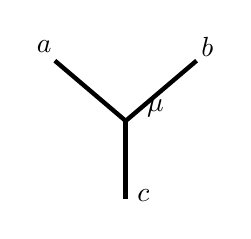
\begin{tikzpicture}[scale=0.9,baseline={(0,-0.1)}]
  \draw[ultra thick] (-1,0.85) -- (0,0);
  \draw[ultra thick] (1,0.85) -- (0,0);
  \draw[ultra thick] (0,0) -- (0,-1.1);
  \node at (-1.15,1.05) {$a$};
  \node at (1.15,1.05) {$b$};
  \node at (0.25,-1.05) {$c$};
  \node at (0.42,0.18) {$\mu$};
\end{tikzpicture}
\end{center}
where $\mu=1,\dots,N_{ab}^{\phantom{ab}c}$ labels a basis element.  The convention in this drawing is that the two incoming lines $a,b$ fuse to the outgoing line $c$.  Reversing the orientation of a line replaces it by the dual line $a^\vee$.  Equivalently, all junctions are morphisms in a tensor category.

Physically, a junction is a local topological operator at the point where topological defects meet.  Since the lines are topological, the junction can be moved freely as long as it does not cross other insertions.  But it can carry a finite-dimensional internal label.  These labels are invisible if all fusions are multiplicity-free, but they are essential in general.

\paragraph{Resolution of multi-junctions.}
Now consider four external lines $a,b,c,d$.  The vector space of topological junctions from $a\otimes b\otimes c$ to $d$ can be described in two natural bases.  In the $s$-channel, one first fuses $a$ and $b$ to an intermediate line $e$, and then fuses $e$ with $c$ to $d$:
\begin{equation}
  \bigoplus_e V_{ab}^{\phantom{ab}e}\otimes V_{ec}^{\phantom{ec}d} .
  \label{eq:leftjunctionresolution}
\end{equation}
In the $t$-channel, one first fuses $b$ and $c$ to $f$, and then fuses $a$ with $f$ to $d$:
\begin{equation}
  \bigoplus_f V_{bc}^{\phantom{bc}f}\otimes V_{af}^{\phantom{af}d} .
  \label{eq:rightjunctionresolution}
\end{equation}
Topological invariance says that these are two bases for the same finite-dimensional junction space.  The change-of-basis matrix is the associator, whose components are the $F$-symbols.

\paragraph{Associators and $F$-symbols.}
Fusion is associative only up to a specified isomorphism.  The associator is a natural isomorphism
\begin{equation}
  \alpha_{a,b,c}: (a\otimes b)\otimes c\longrightarrow a\otimes(b\otimes c) .
\end{equation}
Choose bases for all trivalent junction spaces.  Let
\begin{equation}
  \bigl|(ab)c;d,e,\mu,\nu\bigr\rangle,
  \qquad
  \mu\in V_{ab}^{\phantom{ab}e},
  \quad
  \nu\in V_{ec}^{\phantom{ec}d}
\end{equation}
denote the state in the left resolution \eqref{eq:leftjunctionresolution}.  Let
\begin{equation}
  \bigl|a(bc);d,f,\rho,\sigma\bigr\rangle,
  \qquad
  \rho\in V_{bc}^{\phantom{bc}f},
  \quad
  \sigma\in V_{af}^{\phantom{af}d}
\end{equation}
denote the state in the right resolution \eqref{eq:rightjunctionresolution}.  The $F$-symbols are defined by
\begin{equation}
  \bigl|(ab)c;d,e,\mu,\nu\bigr\rangle
  =
  \sum_{f,\rho,\sigma}
  \left[F^{abc}_{d}\right]_{(e,\mu,\nu)}^{(f,\rho,\sigma)}
  \bigl|a(bc);d,f,\rho,\sigma\bigr\rangle .
  \label{eq:Fsymbols}
\end{equation}
Graphically, this is the $F$-move:
\begin{center}
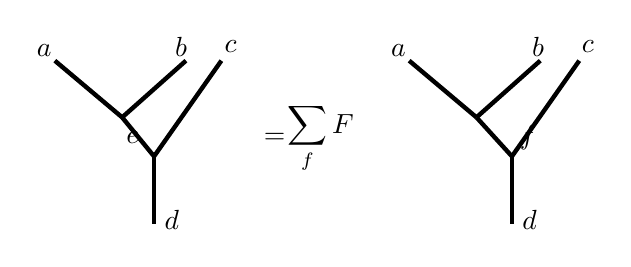
\begin{tikzpicture}[scale=0.9,baseline={(0,-0.2)}]
  \draw[ultra thick] (-2.4,1.1) -- (-1.45,0.3);
  \draw[ultra thick] (-0.55,1.1) -- (-1.45,0.3);
  \draw[ultra thick] (-1.45,0.3) -- (-1.0,-0.25);
  \draw[ultra thick] (-0.05,1.1) -- (-1.0,-0.25);
  \draw[ultra thick] (-1.0,-0.25) -- (-1.0,-1.2);
  \node at (-2.55,1.25) {$a$};
  \node at (-0.62,1.3) {$b$};
  \node at (0.08,1.3) {$c$};
  \node at (-1.3,0.02) {$e$};
  \node at (-0.75,-1.15) {$d$};
  \node at (0.7,0) {$=$};
  \node at (1.35,0) {$\displaystyle\sum_f F$};
  \draw[ultra thick] (2.6,1.1) -- (3.55,0.3);
  \draw[ultra thick] (4.45,1.1) -- (3.55,0.3);
  \draw[ultra thick] (5.0,1.1) -- (4.05,-0.25);
  \draw[ultra thick] (3.55,0.3) -- (4.05,-0.25);
  \draw[ultra thick] (4.05,-0.25) -- (4.05,-1.2);
  \node at (2.45,1.25) {$a$};
  \node at (4.42,1.3) {$b$};
  \node at (5.12,1.3) {$c$};
  \node at (4.28,0.02) {$f$};
  \node at (4.3,-1.15) {$d$};
\end{tikzpicture}
\end{center}
In a multiplicity-free category, where each $N_{ab}^{\phantom{ab}c}$ is $0$ or $1$, the $F$-symbols reduce to numbers
\begin{equation}
  \left[F^{abc}_{d}\right]_{e}^{f} .
\end{equation}
With multiplicities, they are honest matrices implementing the isomorphism
\begin{equation}
  \bigoplus_e V_{ab}^{\phantom{ab}e}\otimes V_{ec}^{\phantom{ec}d}
  \longrightarrow
  \bigoplus_f V_{bc}^{\phantom{bc}f}\otimes V_{af}^{\phantom{af}d} .
  \label{eq:Fasamatrix}
\end{equation}

\paragraph{The pentagon identity.}
The most famous identity is Mac Lane's pentagon.  It says that any two sequences of reassociations of four fused lines give the same result.  In categorical form,
\begin{equation}
  \alpha_{a,b,c\otimes d}\circ \alpha_{a\otimes b,c,d}
  =
  (\id_a\otimes \alpha_{b,c,d})\circ \alpha_{a,b\otimes c,d}\circ(\alpha_{a,b,c}\otimes \id_d) .
  \label{eq:pentagoncategorical}
\end{equation}
This is the cleanest way to remember the identity.  In components, it becomes the equality of two products of $F$-matrices.  In a multiplicity-free convention one common form is
\begin{equation}
  \sum_n
  \left[F^{abc}_{g}\right]_{e}^{n}
  \left[F^{a n d}_{h}\right]_{g}^{m}
  \left[F^{bcd}_{m}\right]_{n}^{p}
  =
  \left[F^{e c d}_{h}\right]_{g}^{p}
  \left[F^{a b p}_{h}\right]_{e}^{m} .
  \label{eq:pentagonmultiplicityfree}
\end{equation}
With multiplicities restored, the same statement is a matrix equation.  A schematic component version is
\begin{equation}
\begin{aligned}
&\sum_{n,\alpha,\beta,\gamma}
\left[F^{abc}_{g}\right]_{(e,\mu,\nu)}^{(n,\alpha,\beta)}
\left[F^{a n d}_{h}\right]_{(g,\beta,\lambda)}^{(m,\gamma,\delta)}
\left[F^{b c d}_{m}\right]_{(n,\alpha,\kappa)}^{(p,\epsilon,\zeta)} \\
&\hspace{3.1cm}=
\sum_{s,\xi,\eta}
\left[F^{e c d}_{h}\right]_{(g,\nu,\lambda)}^{(s,\xi,\eta)}
\left[F^{a b s}_{h}\right]_{(e,\mu,\xi)}^{(m,\delta,\eta)} .
\end{aligned}
\label{eq:pentagonwithmultiplicity}
\end{equation}
The placement of indices depends on the precise conventions for bases and for whether one writes $F$ or $F^{-1}$ in \eqref{eq:Fsymbols}.  The invariant content is always \eqref{eq:pentagoncategorical}.  Physically, the pentagon identity is the statement that the value of a topological defect network does not depend on how we choose to decompose a multi-junction into trivalent junctions.

\paragraph{Unit and triangle identities.}
The invisible defect $\id$ is the tensor unit.  There are natural isomorphisms
\begin{equation}
  \ell_a:\id\otimes a\to a,
  \qquad
  r_a:a\otimes\id\to a .
\end{equation}
They obey the triangle identity
\begin{equation}
  (r_a\otimes \id_b)
  =
  (\id_a\otimes \ell_b)\circ \alpha_{a,\id,b} .
  \label{eq:triangleidentity}
\end{equation}
This is the second standard coherence relation.  In pictures, inserting a trivial line and then reassociating is the same as simply erasing the trivial line.  In a convenient unit gauge, one sets the corresponding unit $F$-symbols to one whenever the fusion spaces are nonzero:
\begin{equation}
  F^{\id a b}_{c}=F^{a\id b}_{c}=F^{a b\id}_{c}=1 .
\end{equation}

\paragraph{Duals, caps, cups, and the zig-zag identities.}
Every oriented topological line has an orientation reversal $a^\vee$.  The duality data are evaluation and coevaluation junctions
\begin{equation}
  \operatorname{ev}_a:a^\vee\otimes a\to\id,
  \qquad
  \operatorname{coev}_a:\id\to a\otimes a^\vee .
\end{equation}
They are the cap and cup in the graphical calculus.  They obey the snake, or zig-zag, identities
\begin{equation}
\begin{aligned}
  (\id_a\otimes \operatorname{ev}_a)\circ
  \alpha_{a,a^\vee,a}\circ
  (\operatorname{coev}_a\otimes \id_a)&=\id_a,\\
  (\operatorname{ev}_a\otimes \id_{a^\vee})\circ
  \alpha^{-1}_{a^\vee,a,a^\vee}\circ
  (\id_{a^\vee}\otimes \operatorname{coev}_a)&=\id_{a^\vee} .
\end{aligned}
\label{eq:zigzag}
\end{equation}
Thus a line may bend around and straighten back out without changing the topological operator.

\paragraph{Bubble and completeness identities.}
Choose a basis $\{\mu\}$ of $V_{ab}^{\phantom{ab}c}$ and a dual basis $\{\mu^*\}$ of $V_{c}^{\phantom{c}ab}$ with respect to the natural pairing obtained by closing the two junctions.  Then the resolution of the identity on the $a\otimes b$ channel is schematically
\begin{equation}
  \id_{a\otimes b}
  =
  \sum_{c,\mu}
  \left(
  a\otimes b\xrightarrow{\ \mu\ } c
  \xrightarrow{\ \mu^*\ } a\otimes b
  \right) .
  \label{eq:junctioncompleteness}
\end{equation}
In pictures this is the statement that a small bubble with an intermediate line $c$ can be expanded in a complete set of junction states.  In a semisimple theory, this is the topological analogue of inserting a complete set of intermediate states in a conformal block decomposition.

A closed contractible loop of a simple line evaluates to its quantum dimension:
\begin{equation}
  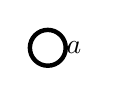
\begin{tikzpicture}[scale=0.35,baseline={(0,-0.05)}]
    \draw[ultra thick] (0,0) circle (0.65);
    \node at (0.95,0) {$a$};
  \end{tikzpicture}
  \;=\; d_a .
  \label{eq:closedloopqdim}
\end{equation}
The quantum dimensions obey
\begin{equation}
  d_a d_b=\sum_c N_{ab}^{\phantom{ab}c}d_c .
  \label{eq:qdimfusion}
\end{equation}
Thus $d_a$ is the positive Frobenius-Perron eigenvector of the fusion matrices.  An invertible line has $d_a=1$.  A genuinely non-invertible line has $d_a>1$ in a unitary theory; the Ising duality line has $d_\sigma=\sqrt2$.

\paragraph{Gauge freedom of $F$-symbols.}
The $F$-symbols are not invariant numbers until bases of junction spaces have been chosen.  A basis change
\begin{equation}
  |ab;c,\mu\rangle
  \longrightarrow
  \sum_{\mu'}
  \left[U_{ab}^{c}\right]_{\mu}^{\phantom{\mu}\mu'}
  |ab;c,\mu'\rangle
\end{equation}
conjugates the corresponding $F$-matrices.  In a multiplicity-free category this reduces to multiplication of the trivalent vertex by a nonzero phase or scalar, and the $F$-symbols change by the associated coboundary.  Physical quantities are invariant under this gauge freedom.

\paragraph{Invertible lines and group cohomology.}
For ordinary group-like symmetry lines, the simple objects are labeled by group elements $g\in G$ and
\begin{equation}
  g\otimes h=gh .
\end{equation}
All junction spaces are one-dimensional when $k=gh$ and vanish otherwise.  The only remaining data are phases in the associator:
\begin{equation}
  \alpha_{g,h,k}: (g h)k\to g(h k),
  \qquad
  \alpha_{g,h,k}=\omega(g,h,k)\in U(1) .
\end{equation}
The pentagon identity becomes the group-cohomology cocycle condition
\begin{equation}
  \omega(h,k,l)\,\omega(g,hk,l)\,\omega(g,h,k)
  =
  \omega(gh,k,l)\,\omega(g,h,kl) .
  \label{eq:groupcocyclecondition}
\end{equation}
A change of basis of the one-dimensional junction spaces changes $\omega$ by a coboundary.  Therefore the associator data for invertible $G$-lines are classified, up to this gauge equivalence, by
\begin{equation}
  [\omega]\in H^3(G,U(1)) .
\end{equation}
This is the categorical way in which a 't Hooft anomaly of an ordinary finite symmetry appears in two dimensions: the symmetry lines still fuse like $G$, but their associator can be anomalous.

\paragraph{No braiding data for ordinary $1+1$d topological symmetry lines.}
The category just described is a fusion category, not a braided fusion category.  This distinction matters.  A topological line in a two-dimensional spacetime is a codimension-one wall.  Parallel walls can be fused, and junctions of walls are local topological operators, but there is no automatic operation that exchanges the order of two walls.  Exchanging two walls would require a crossing, and a crossing is extra local data, not a consequence of topological invariance.  Therefore generic topological symmetry lines in a two-dimensional QFT are not equipped with a canonical commutativity isomorphism
\begin{equation}
  a\otimes b\simeq b\otimes a .
\end{equation}
For these lectures, the core categorical identities are the pentagon identity, the unit/triangle identity, the duality zig-zag identities, and the bubble/completeness identities.

\paragraph{Example: categorical data of the Ising fusion category.}
The Ising fusion category has simple objects $1,\psi,\sigma$ and fusion rules
\begin{equation}
  \psi\otimes\psi=1,
  \qquad
  \psi\otimes\sigma=\sigma\otimes\psi=\sigma,
  \qquad
  \sigma\otimes\sigma=1\oplus\psi .
\end{equation}
All fusion multiplicities are $0$ or $1$.  Therefore the nontrivial $F$-symbols are numbers or small matrices.  A standard gauge choice has
\begin{equation}
  F^{\sigma\sigma\sigma}_{\sigma}
  =\frac{1}{\sqrt2}
  \begin{pmatrix}
    1&1\\
    1&-1
  \end{pmatrix},
  \label{eq:IsingFsss}
\end{equation}
where rows and columns are labeled by the intermediate channels $1,\psi$.  Another standard nontrivial symbol is
\begin{equation}
  F^{\psi\sigma\psi}_{\sigma}=-1,
\end{equation}
while many other $F$-symbols are fixed to $1$ by the unit convention and by fusion with $\psi$.  The fusion rule
\begin{equation}
  \sigma\otimes\sigma=1\oplus\psi
\end{equation}
tells us which intermediate channels are allowed.  The matrix \eqref{eq:IsingFsss} tells us how different resolutions of networks of the duality line are related.  This is the algebraic content behind the Kramers-Wannier relation
\begin{equation}
  \cN\times\cN=\id+\eta .
\end{equation}
The distinction between fusion coefficients and associator data is precisely why non-invertible symmetry is naturally categorical rather than merely group-theoretic.

\subsection{Non-invertible defects: the Ising example}

The two-dimensional critical Ising CFT has three simple topological lines:
\begin{equation}
  \id,\qquad \eta,\qquad \cN .
\end{equation}
Here $\eta$ is the invertible $\Z_2$ spin-flip line.  The line $\cN$ is the Kramers-Wannier duality line.  The fusion rules are
\begin{equation}
  \eta\times\eta=\id,
  \qquad
  \eta\times\cN=\cN\times\eta=\cN,
  \qquad
  \cN\times\cN=\id+\eta .
  \label{eq:IsingFusion}
\end{equation}
The last equation is the simplest example of non-invertibility.  There is no line $\cN^{-1}$ such that $\cN\times \cN^{-1}=\id$.

The slogan is: an invertible topological defect acts as a symmetry operator on the Hilbert space, while a non-invertible topological defect is a more general topological operation.  It may project, dualize, or map between superselection sectors; it need not have an inverse.

\subsection{Application: gapped phases and the action on vacua}

Non-invertible symmetries are especially useful away from criticality.  They give a refined Landau theory of gapped phases.  Let a massive two-dimensional theory have a finite set of isolated vacua
\begin{equation}
  \mathcal V=\{v_i\}_{i=1}^m .
\end{equation}
A topological symmetry line $a$ can be placed along a time slice.  Since the theory is gapped, far from local excitations the only data left are the vacuum labels.  Acting with $a$ on a vacuum therefore gives a formal direct sum of vacua,
\begin{equation}
  a\cdot v_i=\sum_j (n_a)^j_{\ i}\,v_j,
  \qquad
  (n_a)^j_{\ i}\in\Z_{\ge 0} .
  \label{eq:nimrepaction}
\end{equation}
The coefficients are non-negative integers because they count multiplicities of superselection sectors, not probability amplitudes.  Thus the action on vacua is not an ordinary unitary representation on a Hilbert space.  It is a module over the fusion category, or after decategorification a non-negative-integer matrix representation, often called a nimrep.  If
\begin{equation}
  a\times b=\sum_c N_{ab}^{\phantom{ab}c}c,
\end{equation}
then the matrices obey
\begin{equation}
  n_a n_b=\sum_c N_{ab}^{\phantom{ab}c} n_c .
  \label{eq:nimreprelation}
\end{equation}
For ordinary group-like symmetries the matrices $n_g$ are permutation matrices.  Non-invertible symmetries are more general: a line can map one vacuum to several vacua at once.

This immediately gives a useful obstruction.  A phase with a single vacuum would assign a non-negative integer $n_a$ to every simple line.  For the Ising fusion rule \eqref{eq:IsingFusion}, a single-vacuum phase would require
\begin{equation}
  n_\eta=1,
  \qquad
  n_\cN^2=1+n_\eta=2 .
\end{equation}
But there is no integer $n_\cN$ with $n_\cN^2=2$.  Therefore an unbroken Ising-category non-invertible symmetry cannot have a trivially gapped phase with a unique vacuum.  The symmetry either remains gapless, is anomalous in a way that forbids such a phase, or is spontaneously broken so that several vacua appear.

\paragraph{A three-vacuum phase for the Ising fusion category.}
The simplest nontrivial possibility is the regular module.  Label the three vacua by the same symbols as the three simple lines,
\begin{equation}
  v_1,
  \qquad
  v_\psi,
  \qquad
  v_\sigma .
\end{equation}
The Ising symmetry acts by the fusion matrices themselves:
\begin{equation}
\begin{aligned}
  \eta\cdot v_1&=v_\psi,
  &\qquad
  \eta\cdot v_\psi&=v_1,
  &\qquad
  \eta\cdot v_\sigma&=v_\sigma,\\
  \cN\cdot v_1&=v_\sigma,
  &
  \cN\cdot v_\psi&=v_\sigma,
  &
  \cN\cdot v_\sigma&=v_1\oplus v_\psi .
\end{aligned}
\label{eq:IsingRegularModuleAction}
\end{equation}
Equivalently, in the ordered basis $(v_1,v_\psi,v_\sigma)$,
\begin{equation}
  n_\eta=
  \begin{pmatrix}
    0&1&0\\
    1&0&0\\
    0&0&1
  \end{pmatrix},
  \qquad
  n_\cN=
  \begin{pmatrix}
    0&0&1\\
    0&0&1\\
    1&1&0
  \end{pmatrix} .
  \label{eq:IsingRegularModuleMatrices}
\end{equation}
A direct multiplication gives
\begin{equation}
  n_\eta^2=\mathbf 1,
  \qquad
  n_\eta n_\cN=n_\cN n_\eta=n_\cN,
  \qquad
  n_\cN^2=\mathbf 1+n_\eta,
\end{equation}
precisely as required by \eqref{eq:IsingFusion}.  Notice the characteristic non-invertible feature: the duality line does not simply permute the three vacua.  It sends $v_\sigma$ to the sum $v_1\oplus v_\psi$.

\begin{figure}[htbp]
\centering
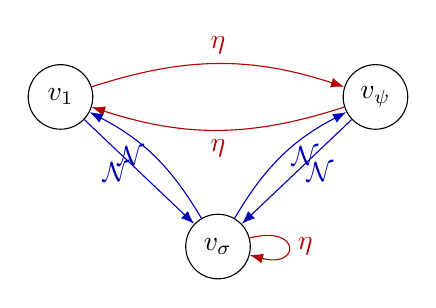
\begin{tikzpicture}[scale=1.0,>=Latex]
  \node[draw,circle,minimum size=0.82cm] (one) at (-2,0) {$v_1$};
  \node[draw,circle,minimum size=0.82cm] (psi) at (2,0) {$v_\psi$};
  \node[draw,circle,minimum size=0.82cm] (sig) at (0,-1.9) {$v_\sigma$};

  \draw[->,red!70!black,bend left=18] (one) to node[above] {$\eta$} (psi);
  \draw[->,red!70!black,bend left=18] (psi) to node[below] {$\eta$} (one);
  \draw[->,red!70!black,loop right] (sig) to node[right] {$\eta$} (sig);

  \draw[->,blue!70!black] (one) to node[left] {$\cN$} (sig);
  \draw[->,blue!70!black] (psi) to node[right] {$\cN$} (sig);
  \draw[->,blue!70!black,bend right=16] (sig) to node[left] {$\cN$} (one);
  \draw[->,blue!70!black,bend left=16] (sig) to node[right] {$\cN$} (psi);
\end{tikzpicture}
\caption{The regular three-vacuum module for the Ising fusion category.  The invertible line $\eta$ permutes vacua, while the non-invertible line $\cN$ acts by a genuine branching rule.}
\label{fig:IsingThreeVacua}
\end{figure}

This is the categorical analogue of a ferromagnet.  For an ordinary finite group, a fully symmetry-broken phase has one vacuum for each group element and the symmetry acts by the regular representation.  For the Ising fusion category, the fully broken phase has one vacuum for each simple object and the symmetry acts by the regular fusion matrices.

This example also illustrates why non-invertible symmetry can distinguish vacua in a way that an ordinary group cannot.  The vacua $v_1$ and $v_\psi$ are exchanged by the invertible line $\eta$, but $v_\sigma$ is fixed by $\eta$ and has a different response to $\cN$.  Thus the vacua are not merely related by a transitive permutation action.

\paragraph{Relation to the tricritical Ising model.}
The three-vacuum phase above is not just an algebraic toy.  Recent lattice constructions with an Ising fusion category symmetry find a phase called the categorical ferromagnet: it fully breaks the Ising fusion category and has three degenerate ground states.  The transition between this categorical ferromagnet and a symmetric critical phase in the ordinary Ising universality class is described by the tricritical Ising CFT with
\begin{equation}
  c=\frac{7}{10} .
\end{equation}
In that realization, perturbing the tricritical Ising fixed point by the relevant symmetry-preserving deformation with the sign pointing into the categorical-ferromagnetic side gives an RG flow to the gapped three-vacuum phase described by \eqref{eq:IsingRegularModuleAction}.  The opposite sign points toward the neighboring symmetric critical Ising phase.  Thus the careful statement is not that every perturbation of the tricritical Ising model produces the three-vacuum phase, but rather that the tricritical Ising fixed point can sit at the transition into this non-invertible-symmetry-breaking gapped phase \cite{BhardwajGappedPhases,RoychowdhuryWangIsingFusion}.


\subsection{Gauging and duality defects}

A very efficient way to generate non-invertible defects is to gauge a finite symmetry in only part of spacetime.  In two dimensions, let a theory $\mathcal T$ have a finite Abelian symmetry $A$.  Gauging $A$ produces $\mathcal T/A$.  If $\mathcal T$ is self-dual under this gauging, then the interface between the ungauged and gauged descriptions becomes a topological duality defect in $\mathcal T$.

For a finite group $A$, the condensation defect obtained by summing over all group defects is
\begin{equation}
  \cC_A=\sum_{a\in A} U_a .
\end{equation}
It obeys
\begin{equation}
  \cC_A\times\cC_A=|A|\,\cC_A .
\end{equation}
After a normalization this is an idempotent projector.  This is one precise sense in which gauging is a non-invertible operation: once one has summed over symmetry bundles, information about the original charge sectors has been lost.

\subsection{Topological defects ending on non-topological defects}

A topological defect may end on a non-topological defect.  The endpoint is a local operator on the non-topological defect.  This is extremely useful physically: it says that a symmetry, or a non-invertible symmetry, constrains the operator spectrum and RG flows of an impurity.

Suppose a codimension-one topological defect $U$ can end on a line defect $L$.  The endpoint operator $\widehat\psi$ lives on $L$:
\begin{equation}
  \partial U=\widehat\psi\in\operatorname{End}(L) .
\end{equation}
Sliding $U$ past defect operators gives selection rules for correlators on $L$.  In anomalous examples, the endpoint algebra may be projective; this is one route to defect anomaly matching.

\begin{exercise}[Topological Ward identity]
Let $J^\mu$ be a conserved current and define
\begin{equation}
  U_\alpha(M)=\exp\left(i\alpha\int_M\star J\right) .
\end{equation}
Show that if $M$ and $M'$ are homologous in the complement of charged
insertions, then $U_\alpha(M)=U_\alpha(M')$ inside correlation functions.
Then show that crossing a charge-$Q$ local operator gives a phase
$e^{i\alpha Q}$.
\end{exercise}

\section{Conformal defects: kinematics}

We now turn to defects that are not topological but sit at a conformal fixed point.

\subsection{Flat conformal defects}

Let the ambient theory be a Euclidean CFT in $d$ dimensions, and let the defect be the flat plane
\begin{equation}
  \Sigma=\{(y^a,z^i): z^i=0\},
  \qquad a=1,\dots,p,
  \qquad i=1,
  \dots,q=d-p .
\end{equation}
The full conformal group $SO(d+1,1)$ is broken to
\begin{equation}
  SO(p+1,1)\times SO(q) .
\end{equation}
Here $SO(p+1,1)$ is the conformal group acting along the defect, while $SO(q)$ rotates the transverse directions.

It is often useful to map a flat defect to a spherical defect.  A line in flat space maps to a circle; a plane maps to a sphere.  This is why expectation values of circular line defects are natural observables.

\subsection{Scalar one-point functions}

Let $\cO$ be a bulk scalar primary of dimension $\Delta$.  In the presence of a flat conformal defect, translations and rotations along the defect imply that
\begin{equation}
  \vev{\cO(y,z)}_{\cD}=f(r),\qquad r=|z| .
\end{equation}
Scale invariance gives
\begin{equation}
  f(\lambda r)=\lambda^{-\Delta}f(r) .
\end{equation}
Therefore
\begin{equation}
  \boxed{\vev{\cO(y,z)}_{\cD}=\frac{a_\cO}{|z|^\Delta}} .
  \label{eq:onepoint}
\end{equation}
This is the simplest diagnostic of a nontrivial conformal defect.  In the trivial defect, $a_\cO=0$ for all non-identity primaries.

For spinning operators, the one-point function is fixed by the preserved group up to a finite number of coefficients.  In particular, the one-point function of a conserved current or stress tensor is strongly constrained and often related to Ward identities.

\subsection{Defect local operators}

A defect local operator $\widehat\cO(y)$ is inserted on $\Sigma$.  It is a primary of $SO(p+1,1)$ and transforms in a representation of the transverse rotation group $SO(q)$.  Its two-point function is
\begin{equation}
  \vev{\widehat\cO_A(y)\widehat\cO_B(0)}
  =\frac{\delta_{AB}}{|y|^{2\widehat\Delta}}
\end{equation}
for an orthonormal basis of defect primaries.

Along a line defect, $p=1$, the defect conformal group is $SO(2,1)$.  The line theory is a one-dimensional conformal theory.  Its primary operators have two-point functions
\begin{equation}
  \vev{\widehat\cO(t)\widehat\cO(0)}=\frac{1}{|t|^{2\widehat\Delta}} .
\end{equation}
Unlike in higher-dimensional CFTs, there is no local stress tensor on an isolated one-dimensional CFT.  The line is conformal because it is embedded in the higher-dimensional CFT.

\subsection{Bulk-defect OPE}

As a bulk operator approaches the defect, it can be expanded in defect operators.  For a scalar bulk primary,
\begin{equation}
  \cO(y,z)=\sum_{\widehat\cO}\frac{b_{\cO\widehat\cO}}{|z|^{\Delta-\widehat\Delta}}
  \widehat\cO(y)+\text{descendants and transverse-spin structures} .
  \label{eq:bulkdefectope}
\end{equation}
More explicitly, if $\widehat\cO$ has transverse spin $\ell$, then the OPE contains a transverse harmonic built from $n^i=z^i/|z|$:
\begin{equation}
  \cO(y,z)\sim \sum_{\widehat\cO_{i_1\cdots i_\ell} } b_{\cO\widehat\cO}\,
  |z|^{\widehat\Delta-\Delta}\,
  n^{i_1}\cdots n^{i_\ell}\,
  \widehat\cO_{i_1\cdots i_\ell}(y)+\cdots .
\end{equation}

\begin{figure}[htbp]
\centering
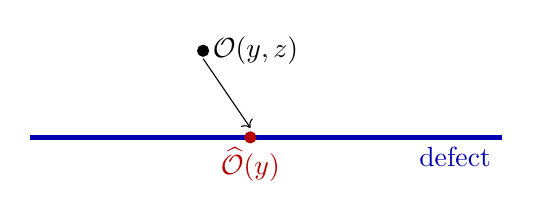
\begin{tikzpicture}[scale=1.0]
  \draw[ultra thick,blue!70!black] (-3,0) -- (3,0);
  \filldraw[black] (-0.8,1.1) circle (2pt) node[right] {$\cO(y,z)$};
  \draw[->] (-0.8,1.0) -- (-0.2,0.12);
  \filldraw[red!70!black] (-0.2,0) circle (2pt) node[below] {$\widehat\cO(y)$};
  \node[blue!70!black] at (2.4,-0.25) {defect};
\end{tikzpicture}
\caption{The bulk-defect OPE replaces a bulk insertion near the defect by a sum of defect-local insertions.}
\end{figure}

The bulk-defect OPE is one of the most important tools in defect CFT.  It is analogous to the ordinary OPE, but it decomposes bulk data into defect data.  In particular, the one-point coefficient $a_\cO$ is the coefficient of the identity defect operator in \eqref{eq:bulkdefectope}.

\subsection{Two-point functions and cross-ratios}

In the presence of a flat defect, a bulk two-point function is not fixed completely by conformal symmetry.  For two scalar primaries,
\begin{equation}
  \vev{\cO_1(x_1)\cO_2(x_2)}_{\cD}
  =\frac{1}{|z_1|^{\Delta_1}|z_2|^{\Delta_2}}\,F(\xi,\eta)
\end{equation}
where $F$ is a function of conformal cross-ratios.  One convenient choice is
\begin{equation}
  \xi=\frac{(y_{12})^2+z_1^2+z_2^2}{2|z_1||z_2|},
  \qquad
  \eta=\frac{z_1\cdot z_2}{|z_1||z_2|} .
\end{equation}
For a boundary, $q=1$, $\eta=\pm1$ and there is only one cross-ratio.

Crossing symmetry equates two decompositions:
\begin{enumerate}
  \item the ordinary bulk OPE $\cO_1\times\cO_2$ followed by one-point functions;
  \item the two bulk-defect OPEs followed by defect two-point functions.
\end{enumerate}
This is the defect bootstrap.

\section{Ward identities and the displacement operator}

\subsection{Broken translations transverse to the defect}

For a flat defect at $z=0$, translations along the defect remain conserved, while translations transverse to the defect are broken.  This is encoded in the Ward identity
\begin{equation}
  \boxed{
  \partial_\mu T^{\mu a}(y,z)=0,
  \qquad
  \partial_\mu T^{\mu i}(y,z)=D^i(y)\,\delta^{(q)}(z) .
  }
  \label{eq:displacementward}
\end{equation}
The operator $D^i$ is the displacement operator.  It is a defect-local operator transforming as a vector of $SO(q)$.

To derive \eqref{eq:displacementward}, consider a small transverse translation localized near the defect:
\begin{equation}
  \delta x^i=\epsilon^i(y,z),\qquad \delta x^a=0 .
\end{equation}
The variation of the bulk action gives
\begin{equation}
  \delta S_{\rm bulk}=-\int \dd^d x\,\partial_\mu \epsilon_i\,T^{\mu i}
  =\int \dd^d x\,\epsilon_i\,\partial_\mu T^{\mu i}
\end{equation}
up to boundary terms.  The variation of the defect insertion under a transverse shift is, by definition,
\begin{equation}
  \delta S_{\rm def}=-\int_{\Sigma}\dd^p y\,\epsilon_i(y,0)D^i(y) .
\end{equation}
Requiring invariance of the path integral for arbitrary $\epsilon_i$ gives \eqref{eq:displacementward}.

\subsection{Protected dimension of the displacement operator}

The stress tensor has dimension $d$.  The delta function $\delta^{(q)}(z)$ has scaling dimension $q$.  Therefore \eqref{eq:displacementward} implies
\begin{equation}
  d+1=\Delta_D+q .
\end{equation}
Since $q=d-p$,
\begin{equation}
  \boxed{\Delta_D=p+1 .}
\end{equation}
This is exact.  For a line defect, $p=1$, so
\begin{equation}
  \Delta_D=2 .
\end{equation}
The two-point function is fixed to be
\begin{equation}
  \vev{D^i(y)D^j(0)}=\frac{C_D\delta^{ij}}{|y|^{2p+2}} .
\end{equation}
The coefficient $C_D$ is a central piece of defect CFT data.  It measures the rigidity of the defect under small transverse deformations.

\subsection{Defect trace Ward identity}

Suppose the defect is perturbed by defect operators:
\begin{equation}
  S=S_{\rm DCFT}+\sum_I \lambda^I\int_\Sigma \dd^p y\,\widehat\cO_I(y) .
\end{equation}
The trace Ward identity has the schematic form
\begin{equation}
  T^\mu_{\ \mu}(x)=\delta^{(q)}(z)\left(\sum_I \beta^I(\lambda)\widehat\cO_I(y)+\cA_{\rm def}\right) .
\end{equation}
The defect is conformal when all defect beta functions vanish and the remaining trace terms are conformal anomalies.  For odd-dimensional defects there is no intrinsic Weyl anomaly, but there may still be universal finite data such as the defect entropy of a line.

\section{Defect RG and perturbation theory}

\subsection{Defect beta functions from OPEs}

Let a $p$-dimensional conformal defect be perturbed by one scalar defect primary:
\begin{equation}
  S=S_*+\lambda_0\int \dd^p y\,\widehat\cO(y),
  \qquad \widehat\Delta=p-\epsilon .
\end{equation}
Define a dimensionless coupling $\lambda=\mu^{-\epsilon}Z_\lambda^{-1}\lambda_0$.  The OPE is
\begin{equation}
  \widehat\cO(y)\widehat\cO(0)\sim \frac{1}{|y|^{2\widehat\Delta}}+\frac{C_{\widehat\cO\widehat\cO\widehat\cO}}{|y|^{\widehat\Delta}}\widehat\cO(0)+\cdots .
\end{equation}
At second order in perturbation theory,
\begin{equation}
  \frac{\lambda_0^2}{2}\int \dd^p y_1\dd^p y_2\,\widehat\cO(y_1)\widehat\cO(y_2)
\end{equation}
contains a short-distance divergence proportional to $\int \widehat\cO$.  Integrating over the relative coordinate $y=y_1-y_2$ in a shell $a<|y|<a e^{\dd \ell}$ gives
\begin{equation}
  \frac{\lambda^2}{2}C_{\widehat\cO\widehat\cO\widehat\cO}
  \int \dd^p Y\,\widehat\cO(Y)
  \int_{a<|y|<a e^{\dd\ell}}\dd^p y\,|y|^{-p+\epsilon}
  =\frac{\lambda^2}{2}C_{\widehat\cO\widehat\cO\widehat\cO}\,\vol(S^{p-1})\dd\ell
  \int \dd^p Y\,\widehat\cO(Y)+O(\epsilon) .
\end{equation}
Thus, up to the conventional sign in the definition of $\lambda$, the beta function is
\begin{equation}
  \boxed{\beta_\lambda=-\epsilon\lambda+\frac{1}{2}\vol(S^{p-1})C_{\widehat\cO\widehat\cO\widehat\cO}\lambda^2+O(\lambda^3).}
  \label{eq:defectbeta}
\end{equation}
For a line defect, $p=1$ and $\vol(S^0)=2$, so the quadratic coefficient is simply $C_{\widehat\cO\widehat\cO\widehat\cO}$ in this normalization.

\subsection{Line-defect entropy and irreversibility}

For a conformal line defect in a $d$-dimensional CFT, map the straight line to a circle $S^1$.  The expectation value
\begin{equation}
  \vev{\cD(S^1_R)}
\end{equation}
contains a scheme-dependent perimeter term.  Away from a fixed point it is therefore better to use the defect entropy
\begin{equation}
  s(R)=\left(1-R\frac{\partial}{\partial R}\right)
  \log\vev{\cD(S^1_R)} .
\end{equation}
The differential operator removes the perimeter term.  At a conformal fixed point $s$ agrees with the universal finite part, which we denote by $\log g$.  The line-defect $g$-theorem states that along a unitary defect RG flow inside a fixed ambient CFT,
\begin{equation}
  s_{\rm UV}>s_{\rm IR}
\end{equation}
unless the flow is trivial.  This generalizes the Affleck-Ludwig boundary entropy theorem to line defects in arbitrary spacetime dimension.

Near a perturbative fixed point one can see the sign directly.  Let the defect
be perturbed by nearly marginal operators $\widehat\cO_I$ with couplings
$\lambda^I$.  Reflection positivity gives a positive metric on the space of
couplings:
\begin{equation}
  G_{IJ}\sim
  \int \dd t\,t^2\,
  \vev{\widehat\cO_I(t)\widehat\cO_J(0)}_{\rm conn},
  \qquad G_{IJ}>0 .
\end{equation}
The defect entropy obeys a gradient formula of the schematic form
\begin{equation}
  \frac{\partial s}{\partial \lambda^I}=-G_{IJ}\beta_R^J+\cdots ,
\end{equation}
where $\beta_R^I=\dd\lambda^I/\dd\log R$ is defined with respect to distance scale.
Therefore along the RG flow,
\begin{equation}
  \frac{\dd s}{\dd \log R}
  =-G_{IJ}\beta_R^I\beta_R^J\le 0 .
\end{equation}
The exact theorem is nonperturbative and can be formulated using relative entropy.

\begin{exercise}[Fixed point from a relevant line perturbation]
Take a line defect perturbed by a scalar of dimension $1-\epsilon$ and beta function $\beta=-\epsilon\lambda+C\lambda^2+O(\lambda^3)$.  Assuming $C>0$, find the IR fixed point and compute the parametric scaling of $\log g_{\rm UV}-\log g_{\rm IR}$.
\end{exercise}

\section{Localized magnetic-field defects in the critical
\texorpdfstring{$O(N)$}{O(N)} model}

We now begin the advanced part.  The first example is perhaps the simplest
nontrivial line defect one can write in an interacting CFT: take the critical
$O(N)$ model and turn on a magnetic field only along a line.  This is a useful
laboratory because it has a transparent microscopic meaning, it is accessible
in the epsilon and large-$N$ expansions, and the infrared answer is a genuine
defect CFT \cite{CKMPinning}.

\subsection{The defect and the RG flow}

Let $\phi^I$, $I=1,\dots,N$, be the order parameter of the critical $O(N)$
model.  We choose a direction in internal space and insert
\begin{equation}
  S_{\rm def}=h\int \dd\tau\, \phi^N(\tau,\vec x_\perp=0) .
  \label{eq:pinningfield}
\end{equation}
The defect preserves translations along the line and rotations around it, but
it explicitly breaks
\begin{equation}
  O(N)\longrightarrow O(N-1) .
\end{equation}
The coupling has dimension
\begin{equation}
  [h]=1-\Delta_\phi .
\end{equation}
For the Wilson-Fisher fixed point in $2<d<4$, and in particular in $d=3$,
$\Delta_\phi<1$.  Therefore the localized field is a relevant perturbation of
the trivial line.

There is a quick way to see that the endpoint cannot be trivial.  Put the line
on a circle of radius $R$.  In the ultraviolet, $hR^{1-\Delta_\phi}\to0$ and
the line disappears, so
\begin{equation}
  g_{\rm UV}=1 .
\end{equation}
The defect entropy must decrease along the flow.  A nontrivial flow starting
from the identity line must therefore end at
\begin{equation}
  \log g_{\rm IR}<0 .
\end{equation}
In particular, it cannot return to the identity.  This elementary example is
a good illustration of how the line $g$-theorem predicts the existence of an
infrared defect before we solve anything.

At the IR fixed point, the leading one-point function is
\begin{equation}
  \vev{\phi^N(\tau,\vec x_\perp)}=\frac{a_\phi}{r^{\Delta_\phi}},
  \qquad
  \vev{\phi^a}=0,
  \qquad a=1,\dots,N-1 .
\end{equation}
where $r=|\vec x_\perp|$.  The nonzero coefficient $a_\phi$ is genuine defect
CFT data.  The profile is the critical analogue of the magnetization cloud
around a pinned spin.

\subsection{Two protected operators}

The bulk $O(N)$ current $J_\mu^{IJ}$ obeys a modified Ward identity in the presence of the defect.  The unbroken currents $J_\mu^{ab}$ remain conserved.  The broken currents $J_\mu^{aN}$ satisfy
\begin{equation}
  \partial_\mu J^{\mu,aN}(x)
  =\delta^{(d-1)}(\vec x_\perp)\,\widehat t^a(\tau) .
  \label{eq:tiltward}
\end{equation}
The defect operator $\widehat t^a$ is called a tilt operator.  The current has
dimension $d-1$, its divergence has dimension $d$, and the transverse delta
function has dimension $d-1$.  Therefore
\begin{equation}
  \boxed{\widehat\Delta_t=1 .}
\end{equation}
This argument is exact.  The tilt operator is the internal-symmetry analogue
of the displacement operator.  The latter follows from broken transverse
translations and obeys
\begin{equation}
  \boxed{\widehat\Delta_D=2}
\end{equation}
for any conformal line.  These two protected operators are useful landmarks in
the defect spectrum.

\subsection{The \texorpdfstring{$4-\epsilon$}{4-epsilon} expansion}

Near four dimensions we may describe the bulk fixed point by
\begin{equation}
  S_{\rm bulk}=\int \dd^{4-\epsilon}x\left[
  \frac12(\partial\phi^I)^2
  +\frac{\lambda}{4!}(\phi^I\phi^I)^2\right] .
\end{equation}
The Wilson-Fisher coupling is
\begin{equation}
  \frac{\lambda_*}{(4\pi)^2}
  =\frac{3\epsilon}{N+8}+O(\epsilon^2) .
\end{equation}
At fixed bulk coupling, the leading terms in the defect beta function are
\begin{equation}
  \beta_h=-\frac{\epsilon}{2}h
  +\frac{\lambda}{(4\pi)^2}\frac{h^3}{6}
  +O(\lambda^2) .
  \label{eq:pinningbetah}
\end{equation}
Substituting the bulk fixed point gives an infrared zero at
\begin{equation}
  h_*^2=N+8+O(\epsilon) .
\end{equation}
The two signs of $h_*$ are related by an $O(N)$ transformation.  Notice that
$h_*$ is not small.  The calculation is nevertheless controlled because at
each order in the small bulk coupling one may sum the required defect
insertions to all orders in $h$.

The operator conjugate to $h$ is the lowest $O(N-1)$ singlet on the line.  Its
dimension follows from the slope of the beta function:
\begin{equation}
  \widehat\Delta_{\phi^N}
  =1+\left.\frac{\partial\beta_h}{\partial h}\right|_{h=h_*}
  =1+\epsilon
  -\frac{3N^2+49N+194}{2(N+8)^2}\epsilon^2
  +O(\epsilon^3) .
  \label{eq:pinningSingletDimension}
\end{equation}
It is irrelevant, while the $O(N-1)$ vector is the protected tilt operator of
dimension one.  Thus the defect fixed point is stable: there is no relevant
defect deformation, whether or not we insist on preserving $O(N-1)$.

The same expansion gives
\begin{equation}
  \log g_{\rm IR}
  =-\frac{N+8}{16}\epsilon+O(\epsilon^2) ,
  \label{eq:pinninggEpsilon}
\end{equation}
with precisely the sign demanded by the $g$-theorem.

\subsection{The large-\texorpdfstring{$N$}{N} saddle}

The large-$N$ solution gives a rather different-looking but compatible
description.  Introduce a Hubbard-Stratonovich field $s$ and scale the source
as $h\sqrt N$:
\begin{equation}
  S=\int \dd^dx\left[
  \frac12(\partial\phi^I)^2+\frac12s\,\phi^I\phi^I\right]
  +h\sqrt N\int\dd\tau\,\phi^N(\tau,0) .
\end{equation}
After integrating out the $\phi^I$, the effective action for $s$ is of order
$N$, and the problem becomes classical.  Conformal invariance allows
\begin{equation}
  \vev{s(x)}=\frac{s_0}{r^2},
  \qquad
  \vev{\phi^N(x)}=\frac{\sqrt N\,A}{r^{(d-2)/2}} .
\end{equation}
The equation obeyed by the order-parameter profile fixes
\begin{equation}
  s_0=\frac{(4-d)(d-2)}{4} .
  \label{eq:pinningLargeNSaddle}
\end{equation}
In three dimensions, $s_0=1/4$.  This value is not an arbitrary
inverse-square potential: it is the one for which the profile has exactly the
power required by the defect conformal symmetry.

There is a useful geometrization of this saddle.  In cylindrical coordinates,
\begin{equation}
  \dd s^2=\dd\tau^2+\dd r^2+r^2\dd\Omega_{d-2}^2
  =r^2\left[
  \frac{\dd\tau^2+\dd r^2}{r^2}+\dd\Omega_{d-2}^2\right] .
\end{equation}
After the Weyl transformation, the line defect sits at the boundary of
\begin{equation}
  AdS_2\times S^{d-2} .
\end{equation}
Defect dimensions become masses in $AdS_2$, while transverse spin becomes
angular momentum on the sphere.  The fluctuation problem for $s$ involves a
bubble diagram in this space.  This is technically nontrivial, but conceptually
very clean: the poles of the AdS spectral representation are the dimensions of
defect operators.

\subsection{Three-dimensional predictions}

The epsilon expansion can be combined with the exact two-dimensional endpoint,
while the large-$N$ saddle can be solved directly in $d=3$.  For the lowest
$O(N-1)$ singlet one finds
\begin{equation}
  \widehat\Delta_{\phi^N}\big|_{d=3}
  =
  \begin{cases}
    1.55\pm0.14, & \text{epsilon expansion and two-dimensional data},\\
    1.542\ldots, & N\to\infty .
  \end{cases}
\end{equation}
The near agreement is striking because the two calculations organize the
physics in completely different ways.  At large $N$ one also obtains
\begin{equation}
  \log g_{\rm IR}=-0.153673\,N+O(N^0),
  \qquad
  a_\phi^2=0.55813\,N+O(N^0) .
\end{equation}
The estimates of the leading irrelevant dimension are compatible with Monte
Carlo studies of the Ising pinning defect, and the one-point coefficient is a
natural target for future simulations.

Let us summarize the picture.  A microscopic magnetic field localized on a
few sites becomes a relevant perturbation of the identity line.  The flow ends
at a stable conformal impurity with a magnetization cloud, protected tilt and
displacement operators, and negative defect entropy.  The same object may be
studied perturbatively near four dimensions, semiclassically at large $N$, or
numerically in three-dimensional critical magnets.  This convergence is what
makes the example so useful.

\section{Wilson lines, charged impurities, and screening}

\subsection{Wilson lines as conformal defects}

In a gauge theory, an external particle in representation $R$ of the gauge group defines a Wilson line
\begin{equation}
  W_R(\gamma)=\operatorname{Tr}_R\,P\exp\left(i\int_\gamma A\right) .
\end{equation}
In a conformal gauge theory, a straight Wilson line may define a conformal line defect.  However, this is not guaranteed: charged matter can screen the line.  The Wilson line is then a UV defect that may flow to a different IR defect.

In supersymmetric theories one often adds scalar couplings,
\begin{equation}
  W_R=\operatorname{Tr}_R P\exp\left(i\int A_\mu\dot x^\mu\dd\tau+\int |\dot x|\,\Phi_I n^I\dd\tau\right),
\end{equation}
which may preserve part of the superconformal algebra.

\subsection{A simple screening criterion from inverse-square physics}

We now spell out the elementary radial problem that underlies the screening criterion.  Work in Lorentzian signature and put a straight electric line on the time axis.  Let
\begin{equation}
  x^\mu=(t,\vec x),
  \qquad
  \vec x=(r,\Omega_{d-2}),
\end{equation}
so that the transverse spatial sphere is $S^{d-2}$.  The line is at $r=0$.  A charged scalar of charge $q$ couples through
\begin{equation}
  D_\mu=\partial_\mu-iq A_\mu .
\end{equation}
Near a static electric line, the conformally invariant Coulomb background has the form
\begin{equation}
  A_t(r)=\frac{a}{r},
  \qquad
  A_r=A_\Omega=0 .
\end{equation}
The dimensionless parameter that controls the radial problem is
\begin{equation}
  \boxed{\kappa\defeq q a .}
  \label{eq:kappaDefinitionWilsonLine}
\end{equation}
Equivalently,
\begin{equation}
  q A_t(r)=\frac{\kappa}{r} .
\end{equation}
In four-dimensional Maxwell theory with action normalized as
\begin{equation}
  S_{\rm Maxwell}=-\frac{1}{4e^2}\int F_{\mu\nu}F^{\mu\nu},
\end{equation}
a Wilson line of electric charge $Q$ produces, up to a sign convention for $A_t$,
\begin{equation}
  A_t(r)=\frac{e^2 Q}{4\pi r},
  \qquad
  \kappa=\frac{q e^2 Q}{4\pi} .
  \label{eq:kappaQED4}
\end{equation}
For a non-Abelian Wilson line whose long-distance electric field lies in the Cartan, $qQ$ is replaced by the pairing between the scalar weight and the electric charge vector of the line.  The sign of $\kappa$ is not important for the near-line instability below; the indicial equation depends on $\kappa^2$.

Consider a free massless charged scalar in this fixed background,
\begin{equation}
  D_\mu D^\mu \Phi=0 .
\end{equation}
With metric $(-,+,\dots,+)$ this is
\begin{equation}
  \left[-D_t^2+\nabla_{\vec x}^2\right]\Phi=0 .
\end{equation}
Separate variables by writing
\begin{equation}
  \Phi(t,r,\Omega)=e^{-i\omega t}\,Y_{\ell m}(\Omega)\,\psi_\ell(r),
\end{equation}
where
\begin{equation}
  \nabla^2_{S^{d-2}}Y_{\ell m}
  =-\ell(\ell+d-3)Y_{\ell m} .
\end{equation}
Since
\begin{equation}
  D_t\Phi=-i\left(\omega+qA_t\right)\Phi
  =-i\left(\omega+\frac{\kappa}{r}\right)\Phi,
\end{equation}
and
\begin{equation}
  \nabla_{\vec x}^2
  =\partial_r^2+\frac{d-2}{r}\partial_r
  +\frac{1}{r^2}\nabla^2_{S^{d-2}},
\end{equation}
the radial equation is
\begin{equation}
  \left[
  \partial_r^2+\frac{d-2}{r}\partial_r
  -\frac{\ell(\ell+d-3)}{r^2}
  +\left(\omega+\frac{\kappa}{r}\right)^2
  \right]\psi_\ell(r)=0 .
  \label{eq:chargedScalarWilsonRadialFull}
\end{equation}
Equivalently,
\begin{equation}
  \left[
  -\partial_r^2-\frac{d-2}{r}\partial_r
  +\frac{\ell(\ell+d-3)}{r^2}
  -\left(\omega+\frac{\kappa}{r}\right)^2
  \right]\psi_\ell(r)=0 .
\end{equation}
Near the line, $r\to0$, the terms proportional to $\omega^2$ and $\omega\kappa/r$ are less singular than $\kappa^2/r^2$.  Therefore the leading scale-invariant equation is
\begin{equation}
  \boxed{
  \left[-\partial_r^2-\frac{d-2}{r}\partial_r
  +\frac{\ell(\ell+d-3)}{r^2}
  -\frac{\kappa^2}{r^2}
  \right]\psi_\ell(r)=0 .
  }
  \label{eq:chargedScalarWilsonRadialLeading}
\end{equation}
This is the inverse-square problem.  The centrifugal barrier is
\begin{equation}
  \frac{\ell(\ell+d-3)}{r^2},
\end{equation}
while the electric Coulomb potential contributes the attractive term
\begin{equation}
  -\frac{\kappa^2}{r^2} .
\end{equation}
Thus $\kappa$ measures the strength of the attraction felt by this particular charged field in this particular electric-line background.

Now try
\begin{equation}
  \psi_\ell(r)\sim r^{-\alpha} .
\end{equation}
Substituting into \eqref{eq:chargedScalarWilsonRadialLeading} gives
\begin{equation}
  -\alpha(\alpha+1)+(d-2)\alpha
  +\ell(\ell+d-3)-\kappa^2=0 .
\end{equation}
Equivalently,
\begin{equation}
  \left(\alpha-\frac{d-3}{2}\right)^2
  =
  \left(\ell+\frac{d-3}{2}\right)^2-\kappa^2 .
  \label{eq:WilsonLineIndicialEquation}
\end{equation}
It is useful to define
\begin{equation}
  \nu_\ell^2
  \defeq
  \left(\ell+\frac{d-3}{2}\right)^2-\kappa^2 .
  \label{eq:nuWilsonLine}
\end{equation}
Then
\begin{equation}
  \alpha_\pm=\frac{d-3}{2}\pm \nu_\ell .
\end{equation}
For $\kappa=0$, the regular solution is $\psi_\ell\sim r^\ell$, which corresponds to
\begin{equation}
  \alpha= -\ell
  =\frac{d-3}{2}-\left(\ell+\frac{d-3}{2}\right) .
\end{equation}
Thus the regular branch is the branch with the minus sign in $\alpha_\pm$.

The defect-operator interpretation is also immediate.  A free bulk scalar has dimension
\begin{equation}
  \Delta_\Phi=\frac{d-2}{2},
\end{equation}
and near a line one writes schematically
\begin{equation}
  \Phi(t,r,\Omega)\sim
  \sum_{\widehat\cO}
  r^{\widehat\Delta-\Delta_\Phi}
  Y_{\ell m}(\Omega)\,\widehat\cO_{\ell m}(t) .
\end{equation}
Since $\psi\sim r^{-\alpha}$, the regular branch gives
\begin{equation}
  \widehat\Delta_\ell
  =\Delta_\Phi-\alpha_-
  =\frac12+\nu_\ell .
  \label{eq:WilsonLineScalarDefectDimension}
\end{equation}
As the electric charge of the line is increased, $|\kappa|$ increases and $\nu_\ell$ decreases.  The lowest channel becomes singular first.  The critical value in the $\ell$th partial wave is
\begin{equation}
  |\kappa|=\kappa_{c,\ell}
  \defeq \ell+\frac{d-3}{2} .
  \label{eq:kappacWilsonLine}
\end{equation}
For the $s$-wave in four spacetime dimensions this is
\begin{equation}
  \kappa_{c,0}=\frac12 .
\end{equation}
When $\nu_\ell^2>0$, the two radial powers are real and scale-invariant boundary conditions can be imposed at the line.  At $\nu_\ell=0$ the two powers collide.  When $\nu_\ell^2<0$, the exponents become complex:
\begin{equation}
  \psi\sim r^{-(d-3)/2}\exp\left(\pm i |\nu_\ell|\log r\right) .
\end{equation}
This is the inverse-square-potential instability, or fall to the center.  In the gauge-theory language it means that the electric line is strong enough to pull charged matter toward the defect.  The resulting cloud screens the original Wilson line.

This radial derivation captures the universal mechanism behind fixed-point annihilation and screening of Wilson lines: as the line charge is varied, a defect operator dimension approaches marginality, two defect fixed points collide, and beyond the collision a screening scale is generated.


\subsection{Defect fixed-point merger}

In this subsection $\kappa$ denotes the positive Coulomb strength $|\kappa|$ in the most dangerous partial wave, and $\kappa_c$ is the corresponding critical value \eqref{eq:kappacWilsonLine}.  The boundary coupling $\lambda$ may be thought of as a short-distance parameter specifying how the two radial solutions are mixed at the line.  Near the collision,
\begin{equation}
  \nu_\ell^2=\kappa_c^2-\kappa^2
  \simeq 2\kappa_c(\kappa_c-\kappa),
\end{equation}
so a beta function written in terms of $\kappa-\kappa_c$ is equivalently an expansion in the parameter that changes the sign of $\nu_\ell^2$.

A universal beta function near a fixed-point merger is
\begin{equation}
  \beta_\lambda=a(\kappa-\kappa_c)+b\lambda^2+\cdots,
  \qquad a b>0 .
\end{equation}
For $\kappa<\kappa_c$ there are two real fixed points,
\begin{equation}
  \lambda_\pm=\pm\sqrt{\frac{a(\kappa_c-\kappa)}{b}} .
\end{equation}
At $\kappa=\kappa_c$ they merge.  For $\kappa>\kappa_c$ there is no real fixed point and RG running generates the scale
\begin{equation}
  \Lambda_{\rm IR}\sim \Lambda_{\rm UV}\exp\left(-\frac{\pi}{\sqrt{ab(\kappa-\kappa_c)}}\right) .
\end{equation}
This Miransky/BKT-type scaling appears in screening clouds around sufficiently large Wilson lines.


\section{'t Hooft lines: marginal operators and non-Abelian instabilities}

The discussion of Wilson lines has a magnetic cousin.  A Wilson line is an electric impurity: it fixes the electric flux sourced by an infinitely heavy charged particle.  A 't Hooft line is a magnetic impurity: it fixes a monopole-like singularity for the gauge field along the line.  In four-dimensional conformal gauge theories both are line defects, and both can have nontrivial defect RG flows.  The main lesson from the work with Aharony, Cuomo, Mezei, and Raviv-Moshe is that one should analyze these lines as DCFTs: expand the bulk fields in the singular background, identify the induced defect operators, and ask which of them are marginal, relevant, or unstable \cite{AharonyWilsonLines,AharonyWilsonLinesLong}.

We will describe two complementary phenomena:
\begin{itemize}
  \item in Abelian QED, charged fermions in a monopole background produce defect fermion modes of dimension $1/2$, hence gauge-invariant bilinears of dimension $1$; these are the marginal operators associated with self-adjoint boundary conditions at the magnetic line;
  \item in non-Abelian gauge theory, the off-diagonal gauge bosons are charged spin-one fields in the monopole background.  Their gyromagnetic coupling turns the centrifugal barrier into an attractive inverse-square potential.  For sufficiently large magnetic charge, and already for the minimal $SU(2)$ 't Hooft line, this produces a fall-to-the-center instability interpreted as $W$-boson condensation and screening of the magnetic line.
\end{itemize}

\subsection{Definition of an Abelian 't Hooft line}

Consider four-dimensional $U(1)$ gauge theory with matter fields of electric charges $q_i$.  A straight 't Hooft line along the time direction is defined by imposing a magnetic monopole boundary condition on a small sphere linking the line.  In a northern gauge patch, the background potential may be written
\begin{equation}
  A=\frac{n}{2}(1-\cos\theta)\,\dd\varphi,
  \qquad
  F=\frac{n}{2}\sin\theta\,\dd\theta\wedge\dd\varphi .
  \label{eq:thooftlinebackground}
\end{equation}
The flux through the linking sphere is
\begin{equation}
  \int_{S^2}F=2\pi n .
\end{equation}
Dirac quantization requires $q_i n\in\Z$ for every dynamical field of charge $q_i$.  The line is magnetically charged under the magnetic one-form symmetry, whose current is conserved by the Bianchi identity,
\begin{equation}
  \dd F=0 .
\end{equation}
This immediately distinguishes Abelian 't Hooft lines from many Wilson lines.  Electric flux can be screened by dynamical electric charges, but magnetic flux in an Abelian theory cannot be screened by ordinary electric matter.  Therefore the Abelian 't Hooft line cannot flow to the completely trivial line.  It is natural to ask what the corresponding IR DCFT is.

The clean way to answer is to set all matter fields to zero, keep the monopole background \eqref{eq:thooftlinebackground}, and analyze matter fluctuations.  The defect spectrum is read off from the radial falloffs of these fluctuations near the line.

\subsection{Charged scalars: monopole harmonics and absence of scalar marginality}

Let $\Phi$ be a massless complex scalar of electric charge $q$.  In the monopole background, the covariant derivative is
\begin{equation}
  D_\mu=\partial_\mu-iqA_\mu .
\end{equation}
The scalar equation is
\begin{equation}
  D^\mu D_\mu \Phi=0 .
\end{equation}
Separate variables as
\begin{equation}
  \Phi(t,r,\theta,\varphi)=e^{-i\omega t}\frac{R(r)}{r}\,Y_{\mu,\ell m}(\theta,\varphi),
  \qquad
  \mu\defeq \frac{qn}{2} .
\end{equation}
The angular functions are monopole spherical harmonics.  Their covariant angular momentum quantum number obeys
\begin{equation}
  \ell=|\mu|, |\mu|+1, |\mu|+2,\dots .
  \label{eq:monopoleharmonicell}
\end{equation}
The radial equation takes the form
\begin{equation}
  -\frac{\dd^2 R}{\dd r^2}
  +\frac{\ell(\ell+1)-\mu^2}{r^2}R
  =\omega^2 R .
  \label{eq:scalarMonopoleRadialGeneral}
\end{equation}
The lowest angular momentum channel has $\ell=|\mu|$.  In this channel
\begin{equation}
  \ell(\ell+1)-\mu^2=|\mu|=\frac{|qn|}{2},
\end{equation}
so
\begin{equation}
  -R''+\frac{|qn|}{2r^2}R=\omega^2R .
  \label{eq:scalarMonopoleRadialLowest}
\end{equation}
Near the line, the $\omega^2$ term is subleading.  With $R\sim r^s$ one obtains
\begin{equation}
  -s(s-1)+\frac{|qn|}{2}=0,
  \qquad
  s=\frac12\pm\sqrt{\frac14+\frac{|qn|}{2}} .
\end{equation}
The normalizable, stable branch uses the plus sign.  Since the four-dimensional scalar has bulk dimension $\Delta_\Phi=1$ and
\begin{equation}
  \Phi\sim r^{s-1},
\end{equation}
the corresponding defect field has dimension
\begin{equation}
  \widehat\Delta_\Phi=s
  =\frac12+\sqrt{\frac14+\frac{|qn|}{2}} .
\end{equation}
The gauge-invariant scalar bilinear therefore has dimension
\begin{equation}
  \boxed{
  \widehat\Delta_{\Phi^\dagger\Phi}
  =2\widehat\Delta_\Phi
  =1+2\sqrt{\frac14+\frac{|qn|}{2}} .
  }
  \label{eq:scalarBilinearThooftDimension}
\end{equation}
For the minimal nonzero value $|qn|=1$ this gives
\begin{equation}
  \widehat\Delta_{\Phi^\dagger\Phi}=1+\sqrt3>2 .
\end{equation}
Thus scalar matter does not produce a relevant or marginal defect operator on an Abelian 't Hooft line.  This is the opposite of what happens for sufficiently highly charged Wilson lines, where the electric Coulomb potential lowers the dimension of charged bilinears until a fixed-point merger is reached.  The magnetic monopole removes the scalar $s$-wave and produces a repulsive centrifugal barrier.

\subsection{Charged fermions: defect zero modes and marginal bilinears}

The fermion case is more interesting.  Let $\Psi$ be a four-dimensional massless Dirac fermion of charge $q$.  The Dirac equation in the monopole background is
\begin{equation}
  \gamma^\mu D_\mu\Psi=0 .
\end{equation}
The angular modes are spinor monopole harmonics.  In contrast to the scalar case, the lowest spinor harmonics have total angular momentum
\begin{equation}
  j=\frac{|qn|}{2}-\frac12,
  \qquad |qn|>0,
  \label{eq:spinorMonopoleLowestJ}
\end{equation}
with degeneracy $|qn|$.  These are the familiar monopole fermion zero-mode channels.

For these lowest channels the radial Dirac equation reduces to a free first-order system on the half-line,
\begin{equation}
  \frac{\dd G}{\dd r}=E F,
  \qquad
  \frac{\dd F}{\dd r}=-E G .
  \label{eq:fermionRadialFree}
\end{equation}
Equivalently,
\begin{equation}
  H
  \begin{pmatrix}F\\G\end{pmatrix}
  =E\begin{pmatrix}F\\G\end{pmatrix},
  \qquad
  H=\begin{pmatrix}
  0&\frac{\dd}{\dd r}\\[2pt]
  -\frac{\dd}{\dd r}&0
  \end{pmatrix} .
\end{equation}
The important point is that the monopole angular momentum and the spin connection cancel the would-be centrifugal barrier.  The two independent solutions are
\begin{equation}
  F=Ae^{iEr}+Be^{-iEr},
  \qquad
  G=-iAe^{iEr}+iBe^{-iEr} .
\end{equation}
Since the line sits at the end of the half-line $r\ge0$, the Hamiltonian must be made self-adjoint by a boundary condition at $r=0$.  Hermiticity requires the boundary term in
\begin{equation}
  \int_0^\infty\dd r\,\left[\Psi_1^\dagger H\Psi_2-(H\Psi_1)^\dagger\Psi_2\right]
\end{equation}
to vanish.  In terms of $F,G$ this requires the allowed boundary values to form a Lagrangian subspace of the boundary pairing.  For one channel this may be written as
\begin{equation}
  B=e^{i\vartheta+i\pi/2}A,
  \label{eq:fermionSelfAdjointTheta}
\end{equation}
where $\vartheta$ is a real angle.  Changing $\vartheta$ is a local deformation of the 't Hooft line.

The radial solution is constant near $r=0$, and after the standard $1/r$ factor in the four-dimensional spinor decomposition the coefficient $A$ or $B$ is interpreted as a defect fermion of dimension
\begin{equation}
  \widehat\Delta_\chi=\frac12 .
\end{equation}
Therefore fermion bilinears localized on the line have
\begin{equation}
  \boxed{\widehat\Delta_{\chi^\dagger\chi}=1 .}
  \label{eq:fermionBilinearThooftMarginal}
\end{equation}
These are the marginal defect operators in QED.  In the simplest language, they are the operators that change the self-adjoint extension parameter \eqref{eq:fermionSelfAdjointTheta}.  Equivalently, the monopole background reduces the lowest four-dimensional fermion modes to massless one-dimensional boundary degrees of freedom, and their bilinears are classically marginal on a line.

For several Weyl fermions, the same statement is refined as follows.  A four-dimensional left-handed Weyl fermion of electric charge $q_i$ gives, in a monopole background of charge $n$, $nq_i$ left-moving two-dimensional fermions on the $(t,r)$ half-plane if $nq_i>0$, and $|nq_i|$ right-moving fermions if $nq_i<0$.  The number of such modes is $|nq_i|$, matching the degeneracy of the spin $|nq_i|/2-1/2$ representation.  A time-independent and rotationally invariant boundary condition at $r=0$ can exist only when the two-dimensional anomaly obstruction vanishes.  In particular, absence of a gravitational anomaly requires
\begin{equation}
  \sum_{q_i>0}|q_i|-
  \sum_{q_i<0}|q_i|=0,
  \label{eq:thooftNoGravAnomaly}
\end{equation}
for $n>0$.  Gauge invariance of the boundary condition requires cancellation of the corresponding two-dimensional gauge anomaly; this condition is equivalent to the four-dimensional gauge anomaly cancellation condition
\begin{equation}
  \sum_i q_i^3=0 .
\end{equation}
When these anomaly constraints are satisfied, the allowed boundary conditions are described by unitary maps between the left-moving and right-moving zero-mode spaces.  The tangent directions to this space of boundary conditions are precisely marginal fermion bilinears.

One should distinguish tree-level marginality from exact marginality.  In ordinary QED, an axial rotation may appear to shift the angle $\vartheta$ in \eqref{eq:fermionSelfAdjointTheta}.  But the axial symmetry is anomalous in four dimensions, so the corresponding defect operator is not protected; gauge interactions make it marginally irrelevant.  By contrast, if there is a genuine non-anomalous global $U(1)$ symmetry whose background participates in the appropriate two-group structure with the magnetic one-form symmetry, then changing the associated boundary angle is an exactly marginal deformation of the 't Hooft line.  This is the defect version of the statement that conserved currents give protected tilt operators: a genuine continuous symmetry can protect a dimension-one operator on a line.

\subsection{Non-Abelian 't Hooft lines and the spin-one instability}

Now consider a weakly coupled non-Abelian gauge theory in four dimensions.  A 't Hooft line is specified by a magnetic flux in the Cartan subalgebra.  Locally, for each electrically charged fluctuation of Cartan charge $q$, the problem reduces to the Abelian monopole problem with effective product $nq$.  The new ingredient is that the off-diagonal gauge bosons are massless charged spin-one particles.  These are the $W$-bosons of the unbroken Cartan description.

The relevant question is the sign of the effective $1/r^2$ potential for a charged particle of spin $s$ and magnetic moment $g_m$ in the monopole background.  Let the orbital monopole angular momentum be
\begin{equation}
  \ell=\frac{|nq|}{2},\frac{|nq|}{2}+1,\dots .
\end{equation}
The total angular momentum is obtained by coupling this orbital angular momentum to the spin $s$.  The centrifugal barrier matrix contains the ordinary monopole angular momentum term and the magnetic moment coupling,
\begin{equation}
  V=\frac{\ell(\ell+1)-\frac14 n^2q^2-\frac12 nq\,g_m\,\widehat r^a S^a}{r^2} .
  \label{eq:generalSpinMonopolePotential}
\end{equation}
For the short representation with total angular momentum
\begin{equation}
  j=\ell-s,
\end{equation}
which exists when $\ell\ge s$, the spin is locked to the radial direction.  Taking $nq>0$ for definiteness, one has
\begin{equation}
  \widehat r^aS^a=s .
\end{equation}
Choosing the lowest orbital value $\ell=nq/2$, the effective potential becomes
\begin{equation}
  \boxed{
  V_{\rm eff}(r)=\frac{1}{2}\,nq\,(1-g_m s)\,\frac{1}{r^2} .
  }
  \label{eq:shortRepPotential}
\end{equation}
This compact formula contains the whole story.

For scalars, $s=0$, so
\begin{equation}
  V_{\rm eff}=\frac{nq}{2r^2}>0 .
\end{equation}
This is the repulsive barrier found above.  For fermions, $s=1/2$ and $g_m=2$, so
\begin{equation}
  V_{\rm eff}=0 .
\end{equation}
This reproduces the marginal fermion modes.  For vector bosons in weakly coupled Yang-Mills theory, however,
\begin{equation}
  s=1,
  \qquad g_m=2,
\end{equation}
and hence
\begin{equation}
  V_{\rm eff}(r)=-\frac{nq}{2}\frac{1}{r^2} .
  \label{eq:vectorAttractivePotential}
\end{equation}
The short representation needed to obtain this channel exists for $nq\ge2$.  In that case the potential is attractive and supercritical.  To see the pathology directly, write the radial equation schematically as
\begin{equation}
  -R''-\frac{nq}{2r^2}R=\omega^2R .
\end{equation}
Near the origin, $R\sim r^s$ gives
\begin{equation}
  s(s-1)+\frac{nq}{2}=0,
  \qquad
  s=\frac12\pm\frac12\sqrt{1-2nq} .
\end{equation}
For $nq\ge2$ the square root is imaginary.  Equivalently, the would-be defect scaling dimensions become complex.  This is the line-defect version of fall to the center.  The conclusion is that the naive 't Hooft line with such magnetic charge is not a healthy conformal defect at weak coupling.  Instead, the charged vector bosons condense near the line.  The endpoint should be a screened or partially screened magnetic line, depending on the theory and on the global form of the gauge group.

\subsection{The \texorpdfstring{$SU(2)$}{SU(2)} versus
\texorpdfstring{$SO(3)$}{SO(3)} lesson}

The simplest example is $\mathcal N=4$ super-Yang-Mills with Lie algebra $\mathfrak{su}(2)$, but considering the non-supersymmetric, $SO(6)_R$-invariant magnetic line that couples only to the gauge field.  The off-diagonal $W$-bosons have Cartan charge
\begin{equation}
  |q_W|=2
\end{equation}
in the normalization where the minimal $SU(2)$ 't Hooft line has magnetic charge $n=1$.  Therefore
\begin{equation}
  |nq_W|=2 .
\end{equation}
This is exactly the first value for which the spin-one short representation exists, and the attractive potential \eqref{eq:vectorAttractivePotential} is already supercritical.  Thus even the minimal non-supersymmetric $SU(2)$ 't Hooft line is unstable at weak coupling.  The natural interpretation is that a cloud of $W$-bosons forms and screens the line in the infrared.

For the gauge group $SO(3)_+$ the global form of the gauge group changes the lattice of allowed line operators and the normalization of electric charges.  The minimal 't Hooft line has $n=1$, while the $W$-boson charge is effectively
\begin{equation}
  |q_W|=1 .
\end{equation}
Then $|nq_W|=1$, and the dangerous vector short representation does not exist.  The minimal $SO(3)_+$ 't Hooft line is therefore expected to define a good conformal line defect at weak coupling.  Higher magnetic charges have $|nq_W|\ge2$ and are unstable.

This is nicely consistent with one-form symmetry and $S$-duality.  In $SU(2)$ theory, the fundamental Wilson line is protected by the electric $\Z_2$ one-form symmetry, while the magnetic 't Hooft lines are not protected and are screened at weak coupling.  Under $S$-duality, $SU(2)$ is exchanged with $SO(3)_+$; the protected electric Wilson line maps to the minimal magnetic line of $SO(3)_+$, which is precisely the one that survives the weak-coupling instability analysis.  The broad picture is that, as one moves on the conformal manifold, line operators disappear by screening except when protected by the appropriate one-form symmetry.

The moral for the lecture is that 't Hooft lines are not automatically innocuous topological probes.  In a conformal gauge theory they should be treated as genuine line defects.  Their low-energy fate is determined by the spectrum of charged fields in the monopole background.  Scalars are lifted by the monopole barrier, fermions give marginal boundary-condition modes, and charged vector bosons can destabilize the line by an inverse-square attraction.


\section{Crystalline defects and emanant flux at Dirac criticality}

This final example is a bridge between microscopic lattice defects and
continuum defect CFT \cite{EmanantFlux}.

\subsection{From lattice defects to continuum flux}

A disclination or dislocation is a defect of crystalline geometry.
Low-energy Dirac fermions do not couple only to the metric geometry; they also
remember microscopic quantum numbers such as rotation eigenvalues and crystal
momenta.  Consequently a crystalline defect may induce an effective continuum
gauge flux.  This is sometimes called emanant flux.

The continuum description near the defect is a Dirac fermion in an
Aharonov-Bohm background,
\begin{equation}
  \oint A=2\pi\alpha .
\end{equation}
The parameter $\alpha$ is quantized or constrained by crystalline data.  At a
Dirac critical point the defect can be conformal, but the resulting DCFT also
depends on the allowed boundary condition at the flux core.  The bulk theory
alone does not determine that boundary condition.

\subsection{Half flux and a defect conformal manifold}

For a massless Dirac fermion in $2+1$ dimensions with flux $\alpha$, angular
momentum modes behave near the origin as
\begin{equation}
  \psi_m(r,\theta)\sim r^{|m+\alpha|-1/2}
  \quad\text{or}\quad
  r^{-|m+\alpha|+1/2},
\end{equation}
depending on the component and convention.  At half flux, one channel becomes
marginal: both independent solutions are allowed by power counting.  A choice
of self-adjoint extension at the origin then becomes a physical defect
coupling.  At criticality this can produce a conformal manifold of line
defects.

The lesson is simple and useful.  Even when the bulk is free, a defect need not
be trivial.  Microscopic crystalline data determine an emergent flux, while
short-distance physics at the core selects a point on the space of conformal
boundary conditions.


\begin{thebibliography}{99}

\bibitem{ShaoTASI}
S.-H. Shao, ``What's Done Cannot Be Undone: TASI Lectures on Non-Invertible Symmetry,'' arXiv:2308.00747.


\bibitem{BhardwajGappedPhases}
L. Bhardwaj, L. E. Bottini, D. Pajer, and S. Schafer-Nameki, ``Gapped Phases with Non-Invertible Symmetries: (1+1)d,'' SciPost Phys. 18 (2025) 032, arXiv:2310.03784.

\bibitem{RoychowdhuryWangIsingFusion}
S. Roychowdhury and C. Wang, ``Symmetry Breaking Phases and Transitions in an Ising Fusion Category Lattice Model,'' arXiv:2604.20201.

\bibitem{GaiottoGeneralized}
D. Gaiotto, A. Kapustin, N. Seiberg, and B. Willett, ``Generalized Global Symmetries,'' JHEP 02 (2015) 172, arXiv:1412.5148.

\bibitem{AffleckLudwig}
I. Affleck and A. W. W. Ludwig, ``Universal Noninteger Ground-State Degeneracy in Critical Quantum Systems,'' Phys. Rev. Lett. 67 (1991) 161.

\bibitem{FriedanKonechny}
D. Friedan and A. Konechny, ``On the Boundary Entropy of One-Dimensional Quantum Systems at Low Temperature,'' Phys. Rev. Lett. 93 (2004) 030402, arXiv:hep-th/0312197.

\bibitem{CKRLineG}
G. Cuomo, Z. Komargodski, and A. Raviv-Moshe, ``Renormalization Group Flows on Line Defects,'' Phys. Rev. Lett. 128 (2022) 021603, arXiv:2108.01117.

\bibitem{CKMPinning}
G. Cuomo, Z. Komargodski, and M. Mezei, ``Localized Magnetic Field in the $O(N)$ Model,'' JHEP 02 (2022) 134, arXiv:2112.10634.

\bibitem{AharonyWilsonLines}
O. Aharony, G. Cuomo, Z. Komargodski, M. Mezei, and A. Raviv-Moshe, ``Phases of Wilson Lines in Conformal Field Theories,'' Phys. Rev. Lett. 130 (2023) 151601, arXiv:2211.11775.

\bibitem{AharonyWilsonLinesLong}
O. Aharony, G. Cuomo, Z. Komargodski, M. Mezei, and A. Raviv-Moshe, ``Phases of Wilson Lines: Conformality and Screening,'' arXiv:2310.00045.

\bibitem{EmanantFlux}
M. Barkeshli, C. Fechisin, Z. Komargodski, and S. Zhong, ``Disclinations, Dislocations, and Emanant Flux at Dirac Criticality,'' arXiv:2501.13866.

\bibitem{SmoothDefectsBootstrap}
B. Gabai, A. Sever, and D.-L. Zhong, ``Bootstrapping Smooth Conformal Defects in Chern-Simons-Matter Theories,'' JHEP 03 (2024) 055, arXiv:2312.17132.

\end{thebibliography}

\end{document}
